\documentclass[UTF8]{ctexart}
\usepackage{geometry, CJKutf8}
\geometry{margin=1.5cm, vmargin={0pt,1cm}}
\setlength{\topmargin}{-1cm}
\setlength{\paperheight}{29.7cm}
\setlength{\textheight}{25.3cm}

% useful packages.
\usepackage{amsfonts}
\usepackage{amsmath}
\usepackage{amssymb}
\usepackage{amsthm}
\usepackage{enumerate}
\usepackage{graphicx}
\usepackage{multicol}
\usepackage{fancyhdr}
\usepackage{layout}
\usepackage{listings}
\usepackage{float, caption}

\lstset{
    basicstyle=\ttfamily, basewidth=0.5em
}

% some common command
\newcommand{\dif}{\mathrm{d}}
\newcommand{\avg}[1]{\left\langle #1 \right\rangle}
\newcommand{\difFrac}[2]{\frac{\dif #1}{\dif #2}}
\newcommand{\pdfFrac}[2]{\frac{\partial #1}{\partial #2}}
\newcommand{\OFL}{\mathrm{OFL}}
\newcommand{\UFL}{\mathrm{UFL}}
\newcommand{\fl}{\mathrm{fl}}
\newcommand{\op}{\odot}
\newcommand{\Eabs}{E_{\mathrm{abs}}}
\newcommand{\Erel}{E_{\mathrm{rel}}}

\begin{document}

\pagestyle{fancy}
\fancyhead{}
\lhead{楠迪, 3230101283}
\chead{四则混合计算器}
\rhead{2024.12.20}

\section{设计思路}

\Large{为了解决四则混合计算器最核心的运算顺序问题,我将数字和运算符两种字符进行了分类,分为数字栈和运算符栈。}\\
\large
\begin{enumerate}
    \item \textbf{自定义栈模版}:比较常规的栈模版设计,pop 和push函数,部分参考github
    \item \textbf{定义运算符顺序}:分别以0 1 2 3定义加减+ -、乘除* /、乘方以及取负的顺序\\
    \item \textbf{利用tokentype审查表达式的合法性}:记忆上一个入栈的字符类型,并与当前入栈内容对比,若出现数字夹空格,连续两个加法的情况。
    
\end{enumerate}

   \section{表达式解析与评估}
表达式评估器的核心在于将中缀表达式解析为可计算的形式。主要步骤包括:

\begin{enumerate}
    \item \textbf{去除空格}:利用去除输入表达式中的所有空格字符。
    \item \textbf{遍历表达式}:逐字符扫描表达式,识别数字、运算符和括号。
    \item \textbf{处理数字}:将连续的数字字符解析为一个数值,压入栈
    \item \textbf{处理运算符}:根据运算符的优先级,依次弹出
    \item \textbf{处理括号}:遇到左括号时压入运算符栈,遇到右括号时弹出运算符直到遇到左括号。
    \item \textbf{计算结果}:表达式遍历完成后,依次弹出运算符栈中的运算符并进行计算,最终操作数栈中剩下的值即为结果。
\end{enumerate}
\\
\section{额外修改}
实现了科学计数法的输入。

\begin{figure}[!t]
	\centering
	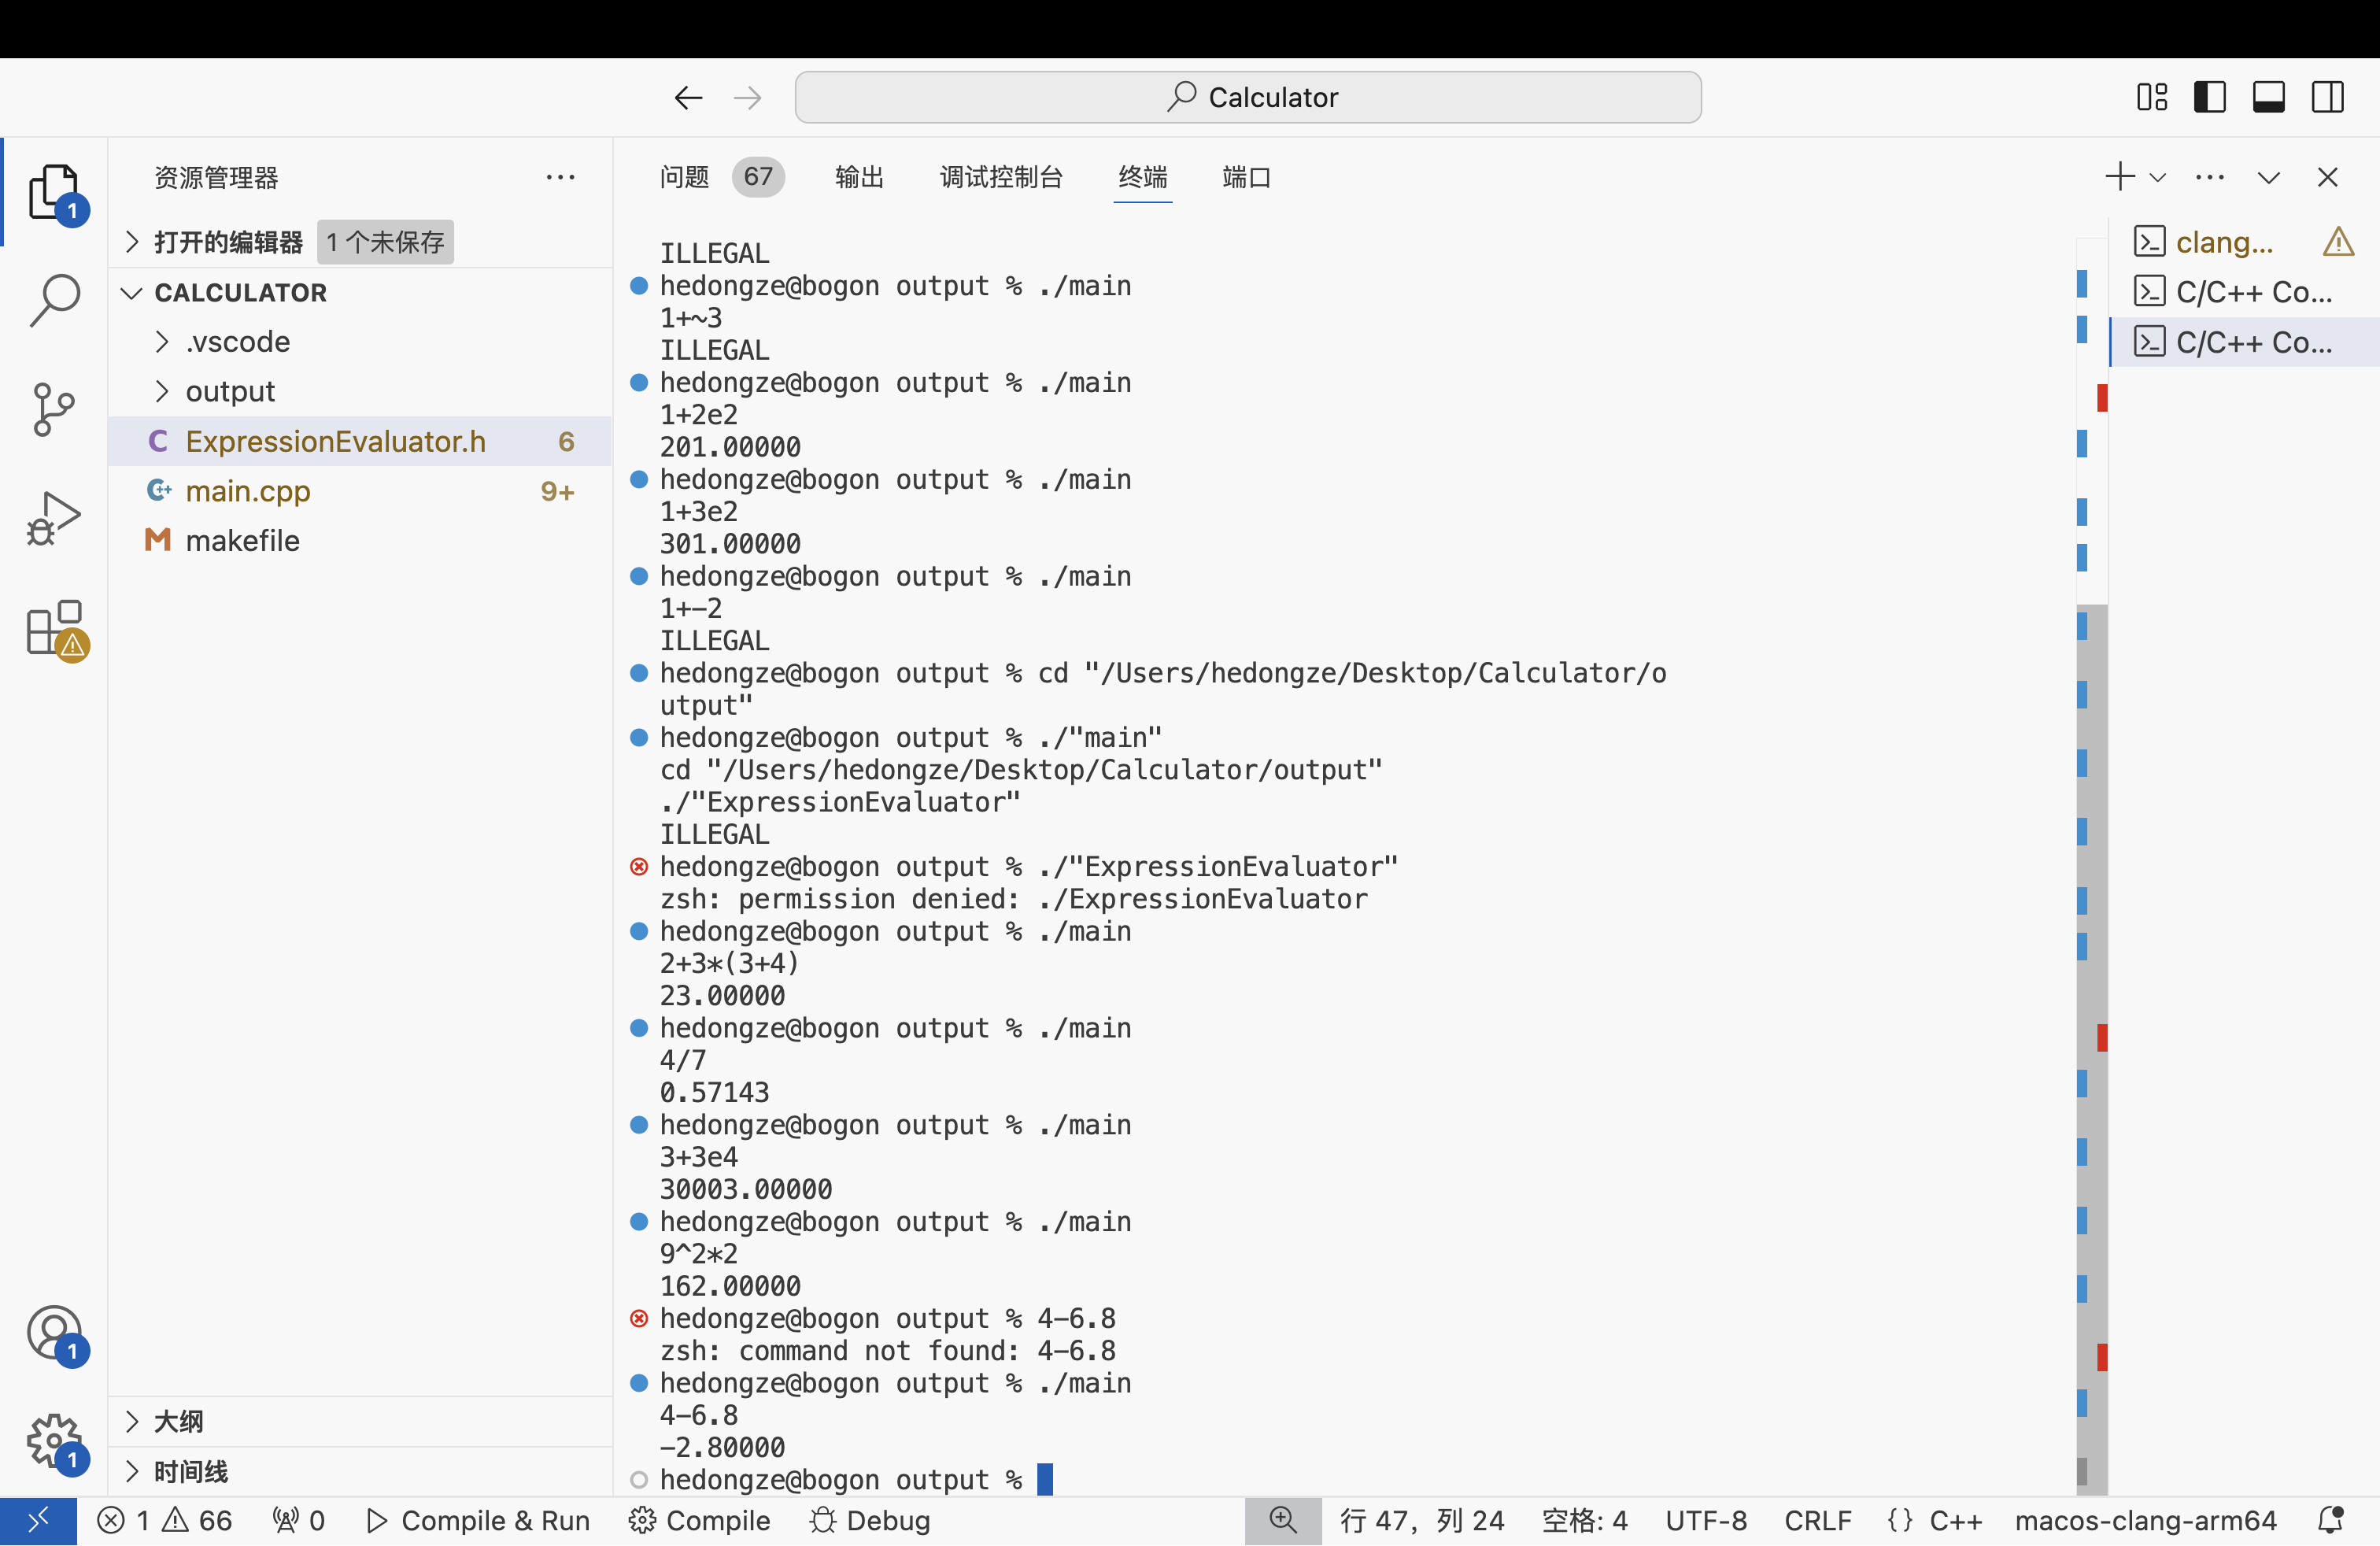
\includegraphics[width=5in]{test.png}
	\caption{Simulation results for the network.}
	\label{fig_sim}
\end{figure}

最后用 valgrind 进行测试,无内存泄露。

\end{document}

%%% Local Variables: 
%%% mode: latex
%%% TeX-master: t
%%% End: 